\section{Overview: Gene tree-species tree models}

Ever since \cite{Zuckerkandl1965a}, researchers have acknowledged that phylogenies reconstructed from homologous gene sequences could differ from species phylogenies.
As molecular sequences accumulated, the link between gene trees and species trees started to be modeled. 
The first models were based on parsimony, and aimed for instance at reconciling a gene tree with a species tree by minimizing the number of events of gene duplication and gene loss. 
In the past dozen years, probabilistic models have been proposed to reconstruct gene trees and species trees in a rigorous statistical framework.
Models and algorithms have quickly grown in complexity, to model biological processes with increasing realism, to accommodate several processes at the same time, or to handle genome-scale data sets.
In this overview we will not detail these models, and we invite the interested reader to take a look at recent reviews (\EG \citep{Szollosi28072014}).

\subsection{Processes of discord}
There are several reasons why a gene tree may differ from a species tree. 
Of course, a gene tree may differ from the species tree just because a mistake was made during the analysis of the gene sequences, at any point in a pipeline going from the sequencing itself to the tree reconstruction.
Such a mistake would produce an incorrect gene tree.
Here we do not mean this kind of discord, but rather discord that comes from a real biological process that generates true gene histories that differ from true species histories.
These processes include gene duplication, gene loss, gene transfer (used loosely here to also include reticulation, hybridization between species), and incomplete lineage sorting (Fig. \ref{fig1}). 
Incomplete lineage sorting will be discussed in more details in the following subsection.

\begin{figure}[h!]
\centering
\fbox{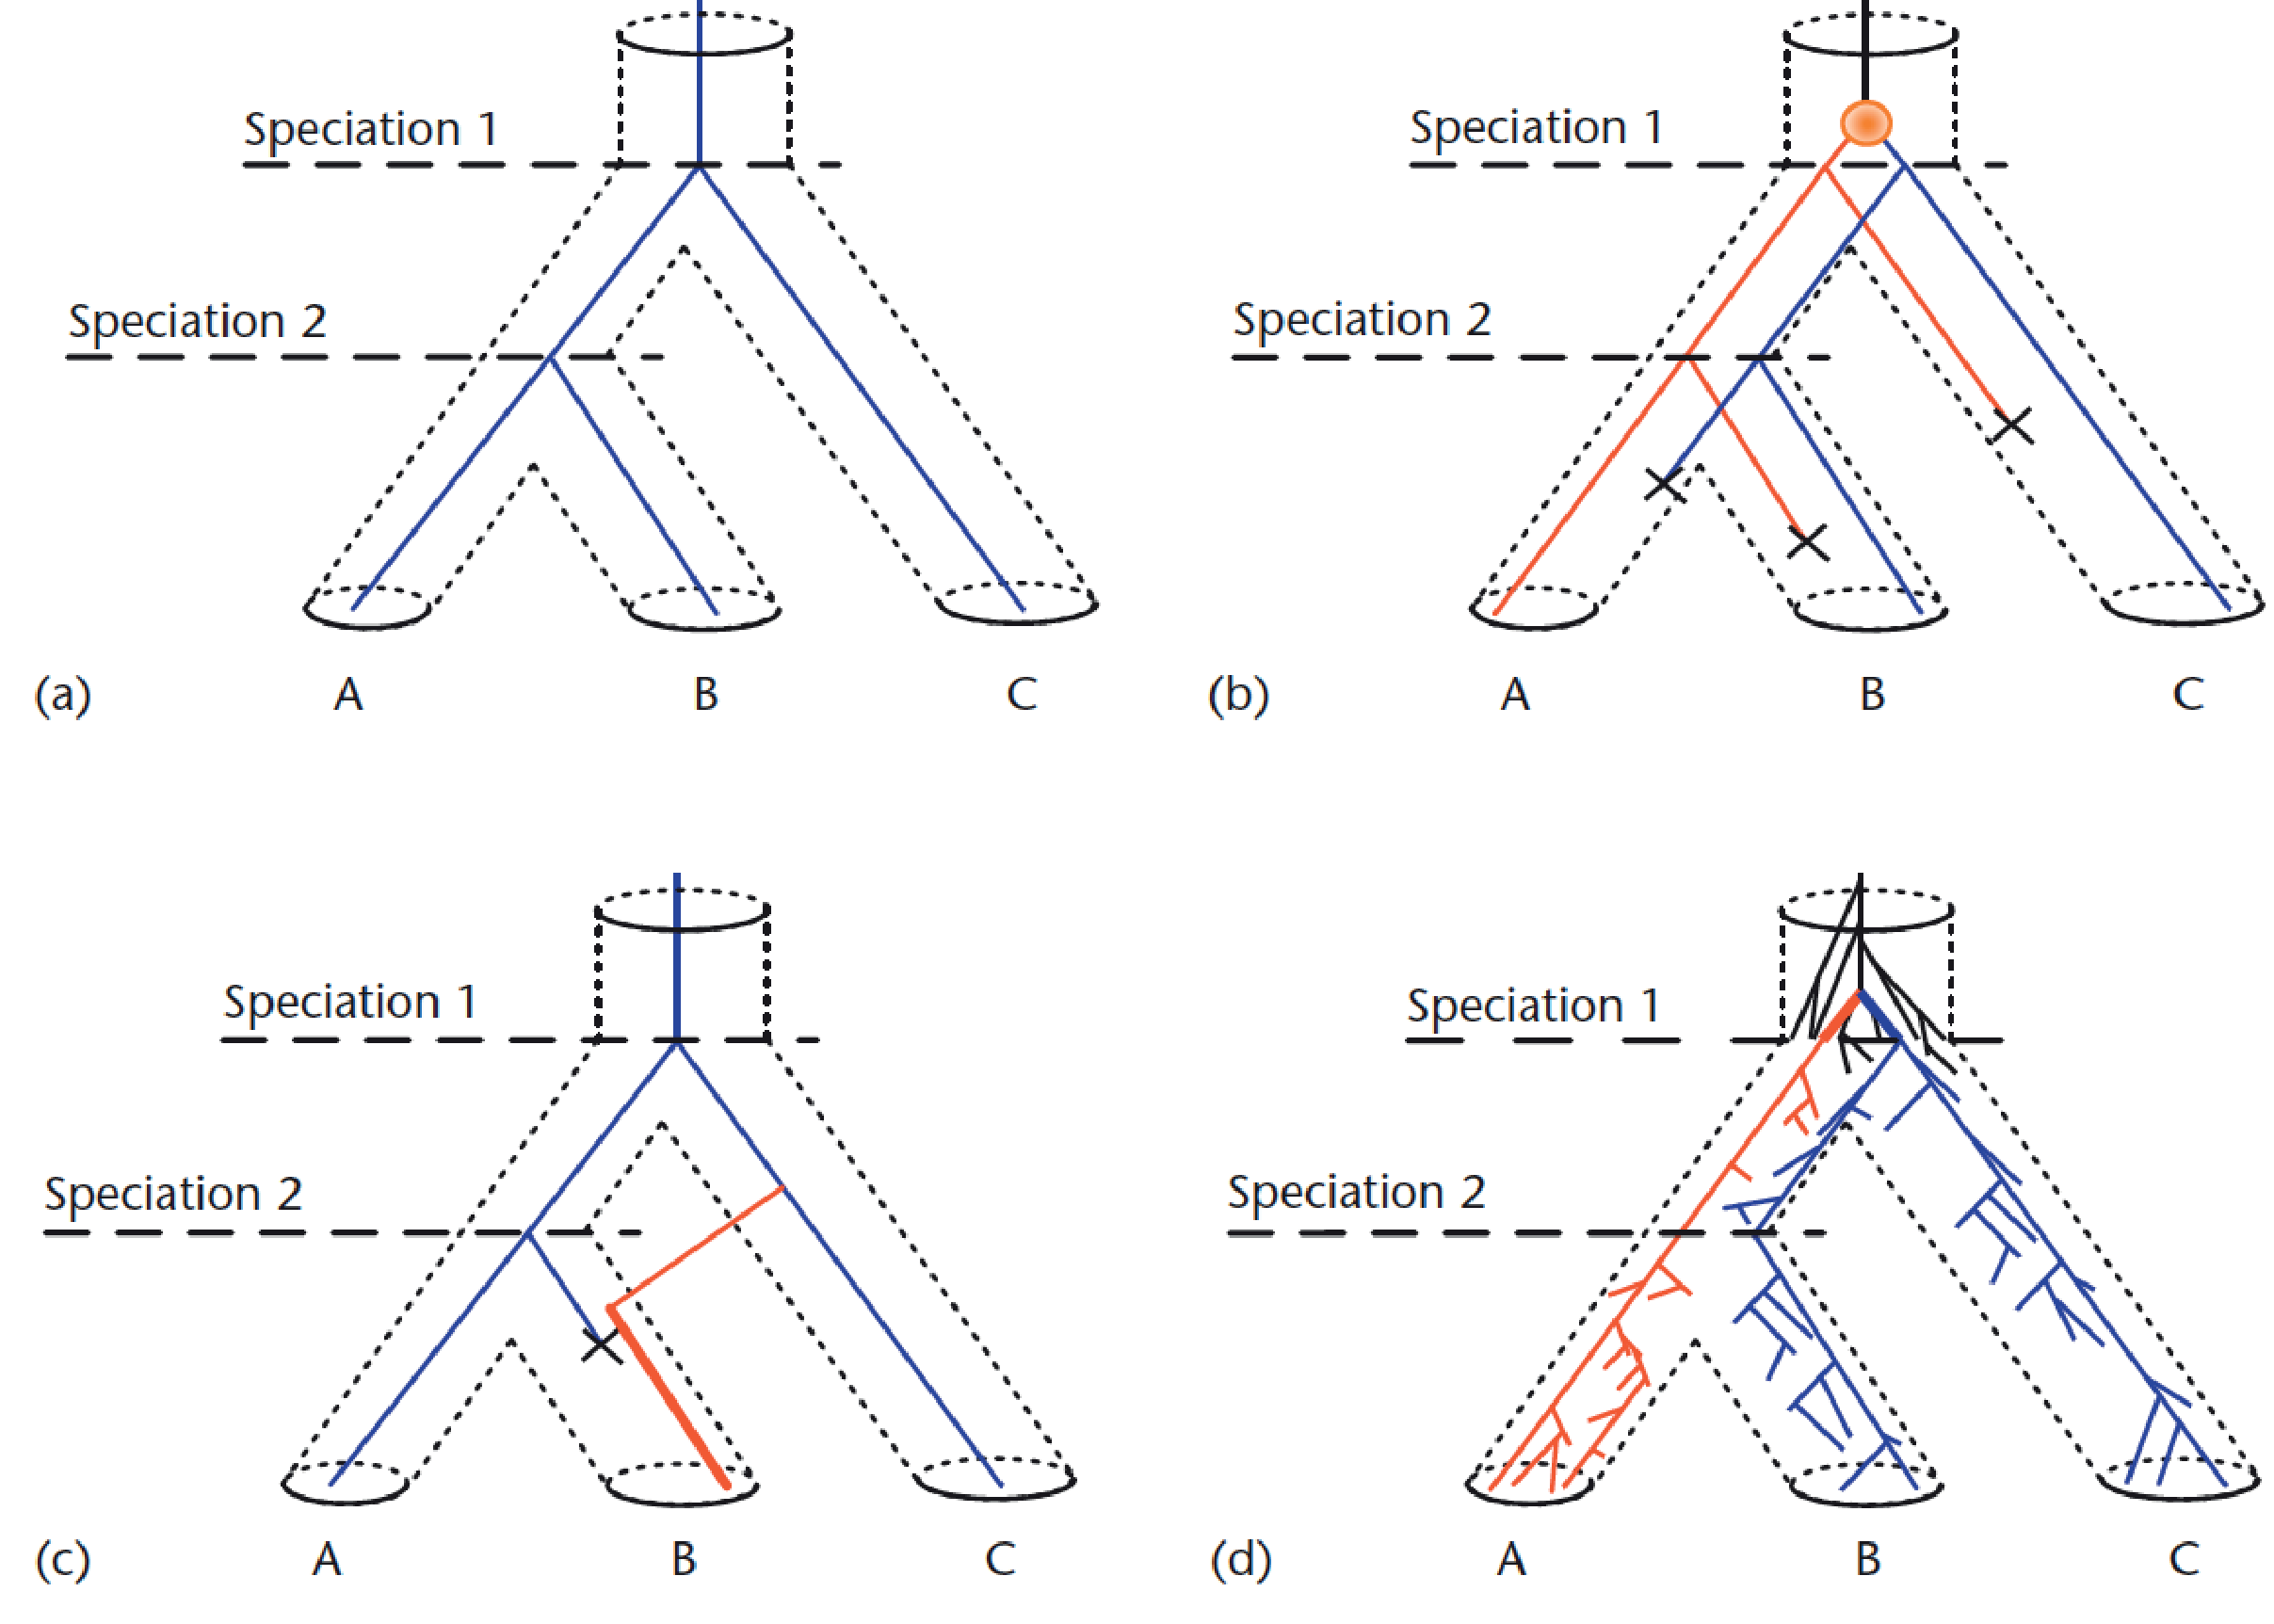
\includegraphics[width=5.8in,angle=0]{\ResourcePath figures/DupTransILS.pdf}}
\caption{\small The processes of discord. The species tree is represented as a tubular structure. Gene trees are blue and red lines running along the species trees. a) A gene tree that perfectly matches the species tree. b) The gene tree and the species tree differ because of gene duplications and losses. c)  The gene tree and the species tree differ because of gene transfer and gene loss. d)  The gene tree and the species tree differ because of incomplete lineage sorting.   [Replicated from Fig.~2 in \citet{Boussau2009}.]}
\label{fig1}
\end{figure}

Fig. \ref{fig1} suggests that for all processes the gene tree can be seen as the product of a branching process operating inside the species tree.
Indeed, all processes are modeled as some type of birth-death process running along the species tree.
For duplication/loss models, birth correspond to gene duplication events, and death to gene loss events.
Transfers can be added to the model by introducing another type of birth, with a child lineage appearing in another branch of the species tree.
Incomplete lineage sorting is also modeled with a birth-death type of model, the coalescent.
All these models can be made heterogeneous, for instance by allowing different sets of parameters for different branches of the species tree.
This is useful to model differences in rates of duplication, loss or transfer among species, or to model different effective population sizes in a species tree.
In \RevBayes~so far only models of incomplete lineage sorting have been implemented (models of duplication and loss and transfer will soon be added).
Thanks to \RevBayes~modular design, there is quite a lot of flexibility in specifying the model, for instance by associating different parameters to different branches of the species tree, or by combining the gene tree-species tree model to other types of models, for instance models of trait evolution, or models of relaxed molecular clock.


\subsection{Gene tree discordance is a problem for species tree reconstruction}
There are several approaches to species tree reconstruction: concatenation and supertree approaches, which have been used for quite some time now, and more recently methods that rely on gene tree-species tree models.\begin{enumerate}
\item Concatenation simply consists in taking all gene alignments, concatenating them into one super alignment, and then analyzing it as if it were a single gene sequence.
Its main assumption is therefore that all sites of all genes have evolved according to the same species tree.
This assumption is not correct because all the processes of discord presented above conspire to make gene trees different from the species tree.
In practice, this matters: simulation studies have found that in the presence of incomplete lineage sorting, in some particular areas of the parameter space, concatenation will often return an incorrect species tree \citep{Leache2011}.
Another example might be found in prokaryotic phylogenetics, where the quest for a tree of life has been difficult, to the point that many doubt that one could find a meaningful species tree representing vertical descent.
Recent models of gene tree evolution incorporating lateral gene transfer allow tackling this question in a more principled way.
\item Supertree approaches differ from concatenation notably by discarding sequence information once individual gene trees have been built.
Contrary to concatenation approaches that combine individual gene alignments, supertree approaches combine individual gene trees to obtain a species tree.
Most supertree methods are not based on an explicit model of the processes causing discordance between gene trees and species tree (although there are exceptions, notably modelling incomplete lineage sorting, see below).
Instead, they aim at finding a tree that would best describe the distribution of gene trees, according to some fairly arbitrary criterion.
In practice, these methods have been found to provide reasonable results in many cases, but in simulations they are usually less accurate than concatenation.
\item Methods that rely on gene tree-species tree models appear very promising as they explicitly model the processes of discord, and can be combined with \EG models of sequence evolution, models of co-evolution between gene trees, models of trait evolution... 
\end{enumerate}


%\bibliographystyle{mbe}
%\bibliography{\ResourcePath refs}

